\section{Introduction}
\label{sec:introduction}

Modern reasoning models such as DeepSeek-R1~\citep{deepseekr1} and the OpenAI o-series~\citep{ElKishky2024OpenAIOS,Chen2025TowardsRE} solve complex tasks through long chains of thought. These traces are not simple token chains: they branch into subgoals, reuse intermediate claims, and revisit earlier derivations~\citep{yeo2025demystify}. Recent probing results further indicate that internal reasoning states are better characterized as dependency graphs than as purely sequential programs~\citep{besta2024graph,zhong2026chains2dags}.

\begin{figure*}[!t]
    \centering
    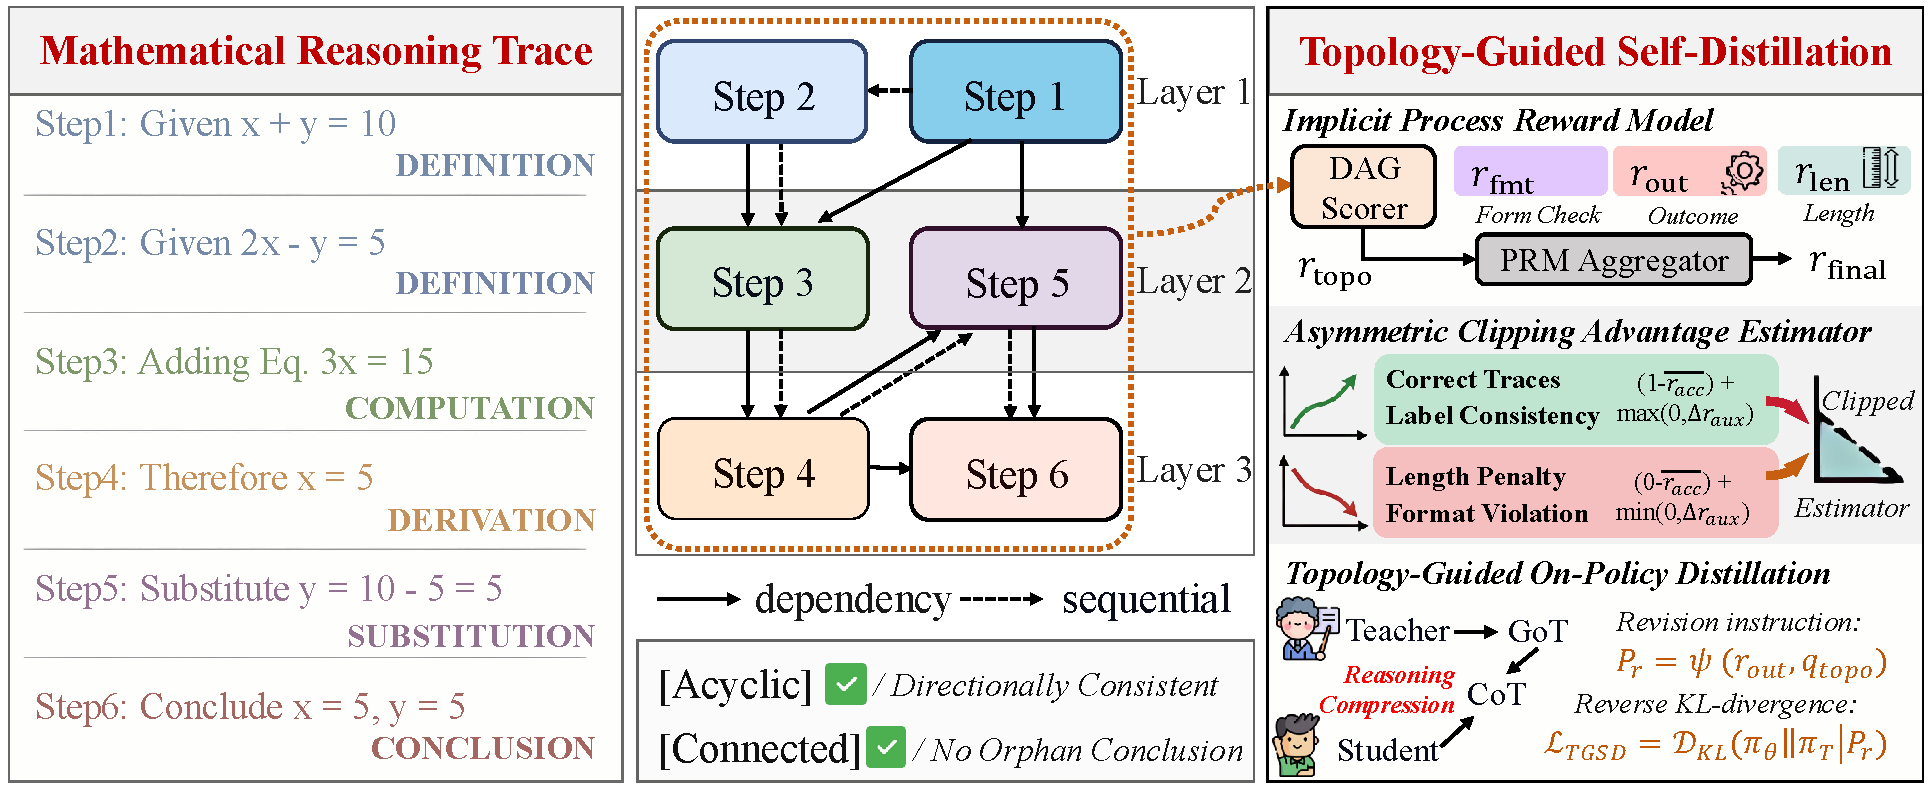
\includegraphics[width=0.96\linewidth]{figures/fig1_topoprm_motivation.pdf}
    \caption{The motivation of \method. A free-form reasoning trace is first turned into an \emph{Implicit Dependency DAG} with typed nodes and edges, which then be judged to drive training stages with topology-aware diagnostics.}
    \label{fig:motivation}
    \end{figure*}

This mismatch between graph-structured reasoning and sequence-only supervision creates three practical failure modes in post-training. First, \emph{dependency omission}: unsupported conclusions can still receive high reward when the final answer is correct. Second, \emph{spurious linearization}: branching reasoning is forced into token-local transitions, which weakens structural credit assignment. Third, \emph{branch redundancy under budget}: outcome-equivalent but structurally inefficient traces are not penalized, which increases truncation sensitivity in long generations. Outcome-only RLVR~\citep{shao2024deepseekmath,lambert2024tulu3,yu2025dapo} and token-level distillation~\citep{agarwal2024gkd,opsdc2026,song2026opdsurvey} do not explicitly model these topology-level distinctions.

Process reward models (PRMs)~\citep{lightman2023lets,wang2024math,thinkprm2025,genprm2026} move supervision from final outcomes to intermediate steps, but most variants still rely on human labels, rollout-heavy annotation pipelines, or learned verifiers that require additional calibration~\citep{luo2024omegaprm,zhang2025qwen25mathprm,yuan2024implicitprm,she2025rprm}. We instead ask whether topology-level supervision can be obtained directly from the trace itself by deterministic extraction.

We propose \method, a topology-aware post-training framework that turns one deterministic dependency-DAG extractor into a shared supervision interface across data construction, reward design, and distillation (Figure~\ref{fig:motivation}). The same DAG diagnostics yield (i) a topology-sensitive \prm, (ii) a hierarchical correctness-first reward optimised with the stratified-clipping advantage estimator \estimation~\citep{liu2026graph}, and (iii) a topology-conditioned on-policy distillation procedure that compresses long traces while preserving dependency structure.

Our contributions are threefold:
\begin{enumerate}[leftmargin=*,itemsep=2pt]
\item \textbf{Topology-as-Reward.} We recast the trace-supervision problem as scoring an implicit dependency DAG, and turn four deterministic graph diagnostics (acyclicity, orphan support, direction consistency, continuity) into a topology-sensitive \prm that needs no human step labels and no learned PRM head.
\item \textbf{\framework: topology-guided self-distillation.} We introduce \framework, a self-distillation framework in which the topology reward acts as a dense token-level signal: a compact student is trained to reproduce a topology-conditioned revision of the teacher trace, simultaneously sharpening reasoning accuracy and compressing reasoning length.
\item \textbf{Empirical recipe.} Under one unified \texttt{transformers} protocol, we benchmark \method against a broad set of open-source baselines on nine math and reasoning datasets (GSM8K, MATH-500, Olympiad, Omni-MATH, AIME~2024, AIME~2025, CNMO~2024, MMLU, GPQA-D), and release a reproducible engineering pipeline built on MS-Swift~\citep{msswift} server-mode GRPO with vLLM rollout and deterministic DAG extraction.
\end{enumerate}
